\documentclass{./../../Latex/tests}

\begin{document}
\thispagestyle{plain}
\myheader{Sample Midterm: Solutions}
\rhead{Sample Midterm: Solutions}
\vspace{0.5em}
\testHeader{70}{20}



\underline{Question 1: Multiple Choice Questions (1 pt each, total 5 pts)}

Select one correct answer unless specified otherwise.
\begin{enumerate}
\item[(a).]	 Below is a scatter plot of two variables $X$ and $Y$. \\
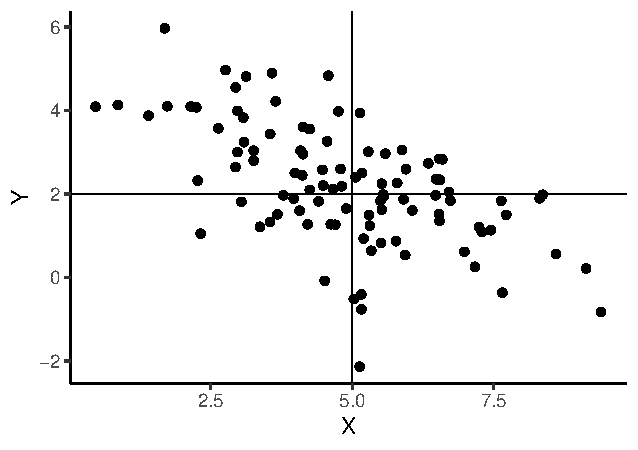
\includegraphics{./../../output/corr_midterm.pdf}\\
What is the correlation between these variables?
\begin{enumerate}
\item[$\square$] $\rho = 0.4$
\item[$\square$] $\rho = -1$
\item[$\text{\rlap{$\checkmark$}}\square$] $\rho = -0.6$
\item[$\square$] $\rho = 0$ \\
\end{enumerate}
%\item[(b).] (Select all that apply) Suppose a survey of 500 people found that 300 of them prefer coffee over tea. Suppose we define a variable X that takes a value of 1 if a person said they prefer coffee and 0 otherwise. The sample mean of $X$ is given as:
%\begin{enumerate}
%\item[$\square$] $1/500(1\cdot 300 + 0\cdot 200) $ 
%\item[$\square$] $(1/500)\sum_{i=1}^{500} X_i$
%\item[$\square$] $300/500$
%\item[$\square$] $1\cdot (3/5) + 0\cdot (2/5) $ \\
%\end{enumerate}
\item[(b).] If the average height in the world is 169 cm with a standard deviation of 6 cm, and my height is 167 cm, how many standard deviations below the mean am I?
\begin{enumerate}
\item[$\square$] $1.24$
\item[$\text{\rlap{$\checkmark$}}\square$] $0.33$
\item[$\square$] $0.67$
\item[$\square$] $2.82$ \\
\end{enumerate}
\newpage
\item[(c).] $X$ and $Y$ are two \textit{independent} random variables. $X$ is a binary variable that takes the value 1 or 0, and $Y$ is a continuous variable. We know that $E(Y|X=1) = 100$, then:
\begin{enumerate}
\item[$\square$] $E(Y|X=0) = 50$
\item[$\text{\rlap{$\checkmark$}}\square$] $E(Y|X=0) = 100$
\item[$\square$] $E(Y|X=0) = 200$
\item[$\square$] We can't say anything about $E(Y|X=0)$ with the above information. \\
\end{enumerate}
\item[(d).] Sample mean $\bar{X}$ is an unbiased estimator for the true population mean $\mu$. Does this mean
\begin{enumerate}
	\item[$\square$] $\bar{X}=\mu$ in all samples.
	\item[$\text{\rlap{$\checkmark$}}\square$] $\bar{X}=\mu$ on average across samples.
	\item[$\square$] $E(\bar{X})=0$
	\item[$\square$] All of the above \\
\end{enumerate}
\item[(e).] (Select all that apply.) Which of the following statements about confidence intervals is true?
\begin{enumerate}
	\item[$\square$] The confidence interval widens as the population variance decreases.
	\item[$\text{\rlap{$\checkmark$}}\square$] The confidence interval widens as the population variance increases.
	\item[$\text{\rlap{$\checkmark$}}\square$] The confidence interval widens as the sample size decreases.
	\item[$\square$] The confidence interval widens as the sample size increases. \\
\end{enumerate}
\end{enumerate}

\newpage 
\underline{\textit{Question 2: Things you can explain (6 pts)}} \\
\begin{enumerate}
\item[(a).] (2 pts) \textit{In most countries across the world mean earnings are greater than median earnings. Why do you think this is true?}  \\~\\
In most countries around the world, average earnings exceed median earnings. This discrepancy arises because a small fraction of people earn exceptionally high salaries, skewing the average upwards. For instance, in the United States, the earnings of the top 5\% account for 28\% of total earnings. \footnote{Estimates from Social Security Data for the year 2017.}  If we plot a histogram of earnings, we will notice that the distribution of earnings is right-skewed. The mean is affected by such outliers as it depends on all values in the data, while the median is less sensitive to extreme values as it only depends on values in the center of the data. \\~\\
\item[(b).] (2 pts) \textit{There is a strong positive correlation between immigrant flows and online job vacancies across metropolitan areas in the US. Does this imply that immigration leads to job creation? } \\~\\
No, this does not imply that immigration leads to job creation because correlation does not imply causation. Immigrants may choose to move to places in response to job vacancies, resulting in a positive correlation between immigrant flows and online job vacancies. This is called reverse casualty. \\~\\
Alternative answer: No, this does not imply that immigration leads to job creation because correlation does not imply causation. Immigrants may settle in areas with [\textit{insert characteristic}] and areas with [\textit{insert characteristic}] also attract more jobs which would result in a positive correlation between immigrant flows and online job vacancies. \\~\\
\item[(c).] (2 pts) \textit{As long as our sample is random (no matter how small or large), the sample mean is going to give us an unbiased estimate of the true population mean. Why do we still care about having a large sample?} \\~\\
We care about having a large sample because the variance of the sample mean given by $\sigma^2/n$ is lower when the sample size $n$ is greater. Unbiasedness implies that, on average, we will get a sample mean equal to the true population mean. It is still very possible to get a sample mean far from the true mean in any given sample; how far depends on the variance of our estimate. Another benefit of having a large sample is that by the Central Limit Theorem, the sample mean distribution in large samples is normal even when the population is non-normal. Knowing the sample mean distribution enables us to construct confidence intervals and perform hypothesis tests.
\end{enumerate}

\newpage 
\underline{Question 3: Voter Turnout (9 pts)} \\

 \textit{We took a random sample of 200 individuals from the US population and asked them whether they voted in the last 
election. We then create a variable $X_i$ that takes value 1 if the individual
voted in the last election and 0 if they did not. 140 individuals said they voted in the last election, while 60 individuals said they didn't. This data is presented in the table below.}\\  
\begin{center}
\setstretch{2}
\begin{tabularx}{\textwidth}{@{}Y| @{}Y |@{}Y| @{}Y| @{}Y| @{}Y@{}}
$(1)$ & $(2)$ & $(3)$ & $(4)$ & $(5)$ & $(6)$ \\
 $X_i$ & $n_i$ & $f_i$ & $f_i X_i$ & $(X_i-\bar{X})^2$ & $f_i (X_i-\bar{X})^2$ \\  \hline
 1 & 140 & \textbf{0.7} & \textbf{0.7} & \textbf{0.09} & \textbf{0.063}\\ \hline
 0 & 60 & \textbf{0.3} & \textbf{0} &  \textbf{0.49} & \textbf{0.147} \\ \hline
Total & 200 & \textbf{1} & \textbf{0.7} & NA & \textbf{0.21} \\ 
\end{tabularx}	
\end{center}
\vspace{2em}


 \begin{enumerate}
 \item[(a).] (2 pts) \textit{Fill in the third and the fourth column of the above frequency distribution table and calculate $\bar{X}$,  the sample mean of $X_i$. Specify the formula you will use and then plug in the values to calculate your answer.} \\
$$\bar{X} = \sum_{i=1}^k f_i X_i = 0.7  $$
\item[(b).] (2 pts) \textit{Your answer in (a) tells us the proportion of individuals in our sample who voted in the last election. Can we directly infer the percentage of the US population that voted in the last election from this answer? Explain.} \\~\\
We cannot directly say that 70\% of the US population voted in the last election. The sample mean is a random variable, and depending on the sample we picked, we could be further or closer to the actual population average. However, since we took a large random sample, the sample mean is normally distributed around the true population mean. So we can construct confidence intervals and perform hypothesis tests to infer something about the true population mean. 
\vspace{1em} \\
\item[(c).] (2 pts) \textit{Fill in the fifth and the sixth column of the above frequency distribution table and calculate $S^2_X$,  the sample variance of $X_i$. Specify the formula you will use and then plug in the values to calculate your answer. } 
$$ S_X^2 = \frac{n}{n-1} \sum_{i=1}^k f_i (X_i-\bar{X})^2 = \frac{200}{199}\cdot 0.21 = 0.211$$
\item[(d).] (3 pts) \textit{You read a headline in LA times that says that the voter turnout last year was 60\%. Test this hypothesis at a 5\% level of significance. State the null and alternative hypothesis, specify the formula for your test statistic, indicate the rejection region, and finally answer whether you reject or fail to reject the null hypothesis. } \\~\\
Null and Alternative Hypothesis: 
$$ H_0: \mu = 0.6 \quad \quad  H_1: \mu \neq 0.6 $$
We calculate the $t$-statistic since we don't know the population variance:
$$ t_0 = \frac{\bar{X}-\mu_0}{S/\sqrt{n}} = \frac{0.7-0.6}{\sqrt{0.211/200}}=\frac{0.1}{0.0325} =3.07 $$ \\
Since $n=200 >100$, we can just look for the critical value in the $Z$ table. At 5\% level of significance, we will reject the null if $|t_0|>1.96$. Here $t_0=3.07$, so we reject the null.

\vspace{5cm}
\end{enumerate}

%\item (2 pts) 
%  \begin{enumerate}
%\item 
%\end{enumerate}
%\item As long as our sample is random (no matter how small or large), the sample mean is going to give us an unbiased estimate for the true mean. Why do we still care about having a large sample?
%\item (1 pt) An estimator $\hat{\theta}$ is an unbiased estimator of $\theta$. If
%\begin{enumerate}
%\item $\hat{\theta} = \theta$ in all samples. 
%\item $\hat{\theta} = \theta$ on average across samples. 
%\item $E(\hat{\theta}) = 0$ 
%\item All of the above
% Show scatter plot and show covariance or why covariance formula works 
%\end{enumerate}





\end{document}